\documentclass[12pt,twoside]{article}
\usepackage{float}
\usepackage[utf8]{inputenc}
\usepackage[spanish]{babel}
\usepackage{amsmath, amssymb}
\usepackage{amsmath}
\usepackage[active]{srcltx}
\usepackage{amssymb}
\usepackage{amscd}

\usepackage[T1]{fontenc}
\usepackage{makeidx}
\usepackage{amsthm}
\usepackage{algpseudocode}
\usepackage{algorithm}
\usepackage{algorithmicx}
\usepackage{graphicx}
\usepackage{vmargin}
\graphicspath{ {images/} }
\renewcommand{\baselinestretch}{1}
\setcounter{page}{1}
\setlength{\textheight}{21.6cm}
\setlength{\textwidth}{14cm}
\setlength{\oddsidemargin}{1cm}
\setlength{\evensidemargin}{1cm}
\setlength{\intextsep}{0pt}
\thispagestyle{empty}
\setpapersize{A4}
\setmargins{2.5cm}       % margen izquierdo
{1.5cm}                        % margen superior
{16.5cm}                      % anchura del texto
{23.42cm}                    % altura del texto
{10pt}                           % altura de los encabezados
{1cm}                           % espacio entre el texto y los encabezados
{0pt}                             % altura del pie de página
{2cm}                           % espacio entre el texto y el pie de página
\date{}
\begin{document}
\centerline{\bf An\'alisis de Algoritmos, Sem: 2019-1, 3CV1, Pr\'actica 1, 29/08/2018}
\centerline{}
\centerline{}
\begin{center}
\Large{\textsc{Pr\'actica 1: Determinaci\'on experimental de la complejidad temporal de un
algoritmo}}
\end{center}
\centerline{}
\centerline{\bf {Hern\'andez Castellanos C\'esar Uriel, Aguilar Garcia Mauricio}}
\centerline{}
\centerline{Escuela Superior de C\'omputo}
\centerline{Instituto Polit\'ecnico Nacional, M\'exico}
\centerline{$uuriel12009u@gmail.com, mauricio.aguilar.garcia.90@gmail.com$}
\newtheorem{Theorem}{\quad Theorem}[section]
\newtheorem{Definition}[Theorem]{\quad Definition}
\newtheorem{Corollary}[Theorem]{\quad Corollary}
\newtheorem{Lemma}[Theorem]{\quad Lemma}
\newtheorem{Example}[Theorem]{\quad Example}
\bigskip
\textbf{Resumen:} El trabajo consiste en mostrar la importancia del análisis de algoritmos, así como la manera experimental de obtener su complejidad.\\
{\bf Palabras Clave:} Algoritmo, Complejidad, Euclides, Suma binaria.
\section{Introducción}
Los algoritmos son de gran importancia tanto en la computación como en nuestra vida diaria, estamos rodeados de ellos, como su definición lo dice: .Es un conjunto prescrito de instrucciones o reglas bien definidas, ordenadas y finitas que permite llevar a cabo una actividad mediante pasos sucesivos que no generen dudas a quien deba hacer dicha actividad.”[1]\\
\\	El análisis de algoritmos se utiliza para conocer la eficacia con la cual el algoritmo que se está analizando realiza su función, esta eficacia se mide respecto al tamaño de la entrada a la que se le ingrese el algoritmo y así obteniendo una función que permita generalizar el tiempo ocupado para terminar su proceso.\\
	Es de gran importancia el análisis, puesto que permite escoger de manera eficaz (y ahorrando la mayor cantidad de recursos posibles) el algoritmo a utilizar dado un problema a resolver.\\
\\	El objetivo de la práctica es reafirmar los conocimiento vistos en clase sobre los métodos de análisis de algoritmos y en específico para esta practica se espera obtener los resultados de manera experimental.
\vspace{50 mm}

\section{Conceptos básicos}
\subsection*{Definición de algoritmo}
Un algoritmo es una secuencia de pasos lógicos necesarios para llevar a cabo una tarea especifica, como la solución de un problema. Los algoritmos son independientes tanto del lenguaje de programación en que se expresan como de la computadora que los ejecuta.
\vspace{10 mm}
\begin{figure}[H]
\centering

\includegraphics[scale=0.1]{img/algoritmo.jpg}
\caption{Algoritmo}
\end{figure}
\subsection*{Algoritmo de Euclides}
El algoritmo de Euclides es un método antiguo y eficaz para calcular el máximo común divisor (MCD). Fue originalmente descrito por Euclides en su obra Elementos. El algoritmo de Euclides extendido es una ligera modificación que permite además expresar al máximo común divisor como una combinación lineal. Este algoritmo tiene aplicaciones en diversas áreas como álgebra, teoría de números y ciencias de la computación, entre otras. Con unas ligeras modificaciones suele ser utilizado en computadoras electrónicas debido a su gran eficiencia.
\begin{figure}[H]
\centering
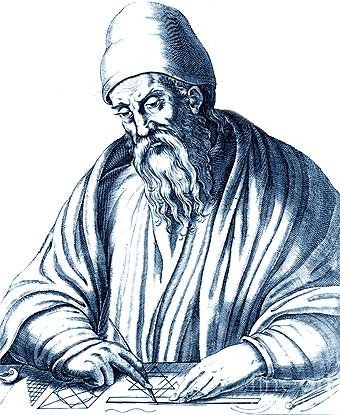
\includegraphics[scale=0.3]{img/euclides.jpg}
\caption{Euclides}
\end{figure}
\subsection*{Algoritmo de ordenamiento por selección}
Consiste en encontrar el menor de todos los elementos del arreglo o vector e intercambiarlo con el que está en la primera posición. Luego el segundo mas pequeño, y así sucesivamente hasta ordenarlo todo. Su implementación requiere $O$($n^2$) comparaciones e intercambios para ordenar una secuencia de elementos. Su funcionamiento se muestra a continuación.

\subsection*{Algoritmo para sumar dos números binarios}
Para hacer la suma binaria se suma columna por columna los ceros o unos y se lleva el acarreo dependiendo del resultado de la suma a continuacion se usa un ejemplo en al fig \ref{sumbinaria} en el cual se demuestra de color negro las pocas operaciones que se usan al sumar bit por bit y como afecta el acarreo: 
\vspace{10 mm}
\begin{figure}[H]
\centering
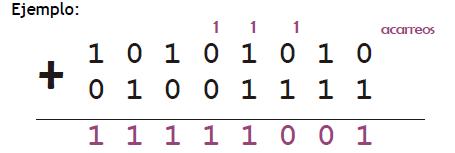
\includegraphics[scale=0.5]{img/Sumbin.png}
\caption{Ejemplo suma binaria}
\label{sumbinaria}
\end{figure}
\subsection*{Notación $\Theta$}
En análisis de algoritmos una cota ajustada asintotica es una función que sirve de cota tanto superior como inferior de otra función cuando el argumento tiende a infinito. Usualmente se utiliza la notación $\Theta$(g(x)) para referirse a las
funciones acotadas por la función g(x).[2]


\subsection*{Notación $O$}
En análisis de algoritmos una cota superior asintotica es una función que sirve de cota superior de otra función cuando el argumento tiende a infinito.

Usualmente se utiliza la notación de Landau: O(g(x)), Orden de g(x), coloquialmente llamada Notación O Grande, para referirse a las funciones acotadas superiormente por la funcion g(x).[2]

\subsection*{Notación $\Omega$}
En análisis de algoritmos una cota inferior asintotica es una función que sirve de cota inferior de otra función cuando el argumento tiende a infinito.
Usualmente se utiliza la notación $\Omega$(g(x)) para referirse a las funciones acotadas inferiormente por la función g(x).[2]

\vspace{100 mm}
\section{Experimentación y Resultados}

\subsection*{Problema uno}
Desarrollar e implementar un algoritmo Suma que sume dos enteros en notacion
binaria bajo las siguientes consideraciones: Dos arreglos unidimensionales A de tama˜no n y
B de tamaño m con k = log2(n) y t = log2(m) almacenarán los números a sumar. La suma
se almacenará en un arreglo C.
\\
\begin{algorithm}[H]
    \caption{Algoritmo para sumar dos números binarios}
      \label{euclides}
      \begin{algorithmic}[1]
          \Procedure{addbinarynumber}{$A,B$}
              \State $sum\gets false$
              \State $carry\gets false$
					\For{$i\gets 0, nbits$}
                      \State $constant\gets nbits-i$
                      \State $bitOne\gets A [constant]$
                      \State $bitTwo\gets B [constant]$
                      \If{$carry$}
                      \If{$bitOne$ \&\& $bitTwo$}
                      \State $carry\gets true$
                      \State $sum\gets true$
                      \ElsIf{$bitOne$ || $bitTwo$}
                      \State $carry\gets true$
                      \State $sum\gets false$
                      \Else
                      \State $carry\gets false$
                      \State $sum\gets true$
                      \EndIf
                      \Else
                      \If{$bitOne$ \&\& $bitTwo$}
                      \State $carry\gets true$
                      \State $sum\gets false$
                      \ElsIf{$bitOne$ || $bitTwo$}
                      \State $carry\gets false$
                      \State $sum\gets true$
                      \Else
                      \State $carry\gets false$
                      \State $sum\gets false$
                      \EndIf
                      \EndIf
                      \If{$sum$}
                      \State $C[constant]\gets true$
                      \EndIf
          \EndFor    
          \EndProcedure
      \end{algorithmic}
  \end{algorithm}
\vspace{10 mm}
El algoritmo desarrollado anteriormente nos realiza la suma de dos números binarios de n bits, se hace uso de dos banderas (sum y carry), en primer lugar iteramos de uno en uno hasta el número de bits de nuestro par de arreglos. Después se comprueba si carry es verdadero, en tal caso que se cumpla realizaremos las condiciones para los diferentes casos, en el caso de que el carry sea falso de igual forma se realizan condiciones para cada caso, pero con el cambio de que las banderas tomarán un distinto valor.
\vspace{10 mm}
\begin{figure}[h]
\centering
\includegraphics[scale=0.6]{img/xd.png}
\caption{Gráfica del algoritmo de suma de dos números binarios}
\label{ejecucionEuclides}
\end{figure}
\vspace{8 mm}
Al implementar el algoritmo se le agregó una variable k para cada linea, con el fin de poder obtener el orden de complejidad por el método de linea por linea, por lo que nuestro resultado fue el mostrado en la figura 4
\vspace{10 mm}
\begin{figure}[H]
\centering
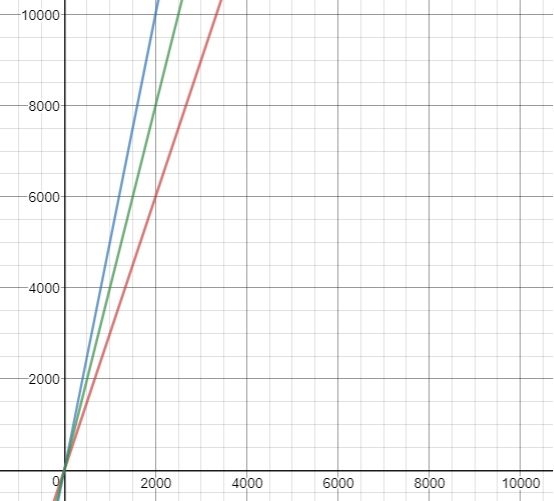
\includegraphics[scale=0.7]{img/propuestas.png}
\caption{Funciones propuestas f1(n) = 5n y f2(n) = 3n}
\label{ejecucionEuclides}
\end{figure}

En la figura 5 se muestran las funciones propuestas que acotan como por la parte inferior y superior a la función que se obtuvo de manera experimental
\vspace{10 mm}

\begin{figure}[H]
\centering
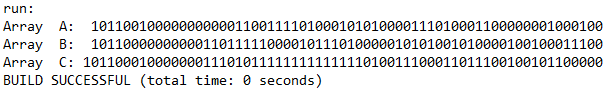
\includegraphics[scale=1.0]{img/numBin_Res.png}
\caption{Ejecucion del algoritmo de suma de dos números binarios}
\label{ejecucionEuclides}
\end{figure}
\vspace{5 mm}
En la figura 6 se muestra la ejecución del programa con dos arreglos de 64 bits que fueron poblados de manera aleatoria.
\subsection*{Problema dos}
Implementar el algoritmo de Euclides para encontrar el mcd de dos números enteros
positivos m y n.
\vspace{5 mm}
\begin{algorithm}
    \caption{Algoritmo de Euclides}
    \label{euclides}
    \begin{algorithmic}[1]
        \Procedure{Euclides}{$m,n$}
            \While{$n\not=0$} 
            \State $m  \bmod n$
			\State $m\gets n$
             \State $n\gets r$
            \EndWhile
        \EndProcedure
    \end{algorithmic}
\end{algorithm}
\vspace{10 mm}

El algortimo de euclides ya que se encarga el calcular el maximo comun divisor,como se observa en la figura \ref{ejecucionEuclides} recibe 2 valores y nos devuelve su MCD con los pasos que hizo el algoritmo para mostrar los resultados en cada linea en la que hubo una operación.
\vspace{10 mm}
\begin{figure}[H]
\centering
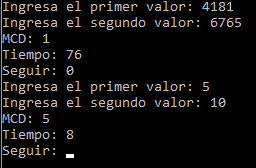
\includegraphics[scale=1.0]{img/Ejecucioneuclides.png}
\caption{Ejecucion algoritmo de euclides}
\label{ejecucionEuclides}
\end{figure}
\vspace{10 mm}
Al implementar el algoritmo ingresamos el peor de sus casos el cual seria la sucesion de fibonacci en el cual se puede apreciar en la figura \ref{graficaEuclides} en la cual se aprecia de color azul el peor caso y con naranja un caso para acotarlo en el cual tambien es la función logaritmica $4\log_{2} (x^2) $.
\vspace{10 mm}
\begin{figure}[H]
\centering
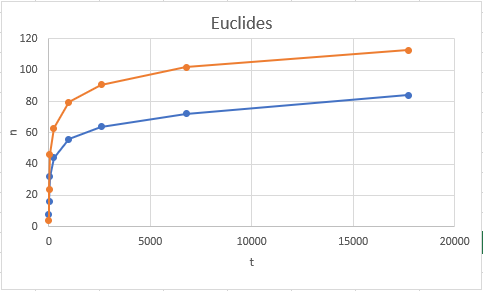
\includegraphics[scale=1.0]{img/Euclides.png}
\caption{Resultados algoritmo de Euclides}
\label{graficaEuclides}
\end{figure}
\vspace{2000 mm}
\section{Conclusiones}
\vspace{10 mm}
\subsection*{Conclusión general}
Para cada algoritmo, son interesantes un par de medidas de complejidad: en el peor caso (que señalamos con la notación O, y en el mejor, para el que utilizamos la notación omega. En especial, suele ser más imprescindible conocer el peor caso, ya que nos da una idea de qué es lo que puede pasar cuando las cosas van realmente mal.\\

Es de gran importancia diseñar nuestros algoritmos de manera adecuada para evitar el uso de recursos computacionales de manera innecesaria.

\subsection*{Aguilar Garcia Mauricio}
En esta práctica me costo mucho trabajo calcular la complejidad del algorimo de Euclides debido a como funciona el modulo, también me sirvió para repasar los temas y me ayudo a comprender la importancia de analizar la complejidad de los algoritmos.\\

Me permitió pensar en como se pueden llegar a generar el peor de los casos y lo útil que es, saber como generar los casos de prueba correctos, lo que nos permite checar el tiempo que deberia de tomar en correr de acuerdo con su complejidad.

\subsection*{Hernández Castellanos César Uriel}
El algoritmo de Euclides, a pesar de su edad, es un algoritmo que prueba su
valor gracias al buen rendimiento que tiene, ya que su complejidad no es la peor de este tipo de algoritmos en el caso del algoritmo de Euclides nos resultó una función logarítmica, además se propuso una función que acotara por la parte superior a la función obtenida de manera experimental.\\

El algoritmo para la suma de dos números binarios que me tocó implementar no representó mayor problema al implementarlo, excepto en el acarreo del último bit que fue donde se me presentaron algunas dificultades. El algoritmo que implementé resultó tener complejidad lineal además, se propusieron dos funciones que acotaron a la función obtenida tanto en la parte inferior como superior.\\

La práctica me permitió conocer la importancia que debemos de tener como ingenieros en diseñar nuestros algoritmos, ya que un mal planteamiento podría conllevar a un mayor costo computacional innecesario.
\vspace{200 mm}

\section{Anexo}
El siguiente algoritmo, es un algoritmo de ordenamiento llamado por selección (SelectSort(A)).
El peor caso se presenta cuando A est\'{a} ordenado de manera decreciente.\\
\begin{tabular}{l l}
\hspace*{1cm}for \emph{j} $ \leftarrow$ 0 to \emph{j} $\leq$ \emph{n -- 2} do
&$c_{1}$\hspace*{0.5cm}$n$\\
\hspace*{1.5cm}\emph{k} $\leftarrow$ \emph{j}
&$c_{2}$\hspace*{0.5cm}$n-1$\\
\hspace*{1.5cm}for \emph{i} $ \leftarrow$ \emph{j + 1} to \emph{i} $\leq$ \emph{n -- 1} do
&$c_{3}$\hspace*{0.5cm}$\displaystyle\sum_{i=0}^{n-1}t_i$\\
\hspace*{2cm}if A[\emph{i}] $\leq$ A[\emph{k}] then
&$c_{4}$\hspace*{0.5cm}$\displaystyle\sum_{i=0}^{n-1}(t_i-1)$\\
\hspace*{2.5cm}\emph{k} $\leftarrow$ \emph{i}
&$c_{5}$\hspace*{0.5cm}$\displaystyle\sum_{i=0}^{n-1}(t_i-1)$\\
\hspace*{1.5cm}Intercambia(A[\emph{j}],A[\emph{k}])
&$c_{6}$\hspace*{0.5cm}$n-1$
\end{tabular}

Sea $t_i$ la cantidad de veces que se ejecuta el for interno.\\
Se tiene que\\
\begin{tabular}{l | l}
$i$& $t_i$\\
\hline
1 &n--1\\
2 &n--2\\
3 &n--3\\
4 &n--4\\
$i$ &n--$i$
\end{tabular}
$\Rightarrow t_i = n - i$\\
$T(n) = c_1n + c_2(n-1) + c_3\displaystyle\sum_{i=0}^{n-1}t_i + c_4\displaystyle\sum_{i=0}^{n-1}(t_i-1)+ c_5\displaystyle\sum_{i=0}^{n-1}(t_i-1)+ c_6(n-1)  $\\
sustituyendo $t_i$\\
$T(n) = c_1n + c_2(n-1) + c_3\displaystyle\sum_{i=0}^{n-1}(n - i) + c_4\displaystyle\sum_{i=0}^{n-1}(n - i-1)+ c_5\displaystyle\sum_{i=0}^{n-1}(n - i-1)+ c_6(n-1)  $
\\simplificando y renombrando las constantes, se tiene\\
$T(n) = an^2 = bn +c = O(n^2)$
\\Cuando el arreglo esta ordenado de manera decreciente, Selection Sort $\in O(n^2)$.

\section{Bibliograf\'ia}

[1]Brassard, Gilles; Bratley, Paul (1997). Fundamentos de Algoritmia. Madrid: PRENTICE HALL.

[2] Introduction to Algorithms, Second Edition by Thomas H. Cormen, Charles E. Leiserson, Ronald L. Rivest, Clifford Stein



\end{document}